\documentclass[11pt]{article}
\usepackage[margin=0.7in]{geometry}
\usepackage[parfill]{parskip}
\usepackage[utf8]{inputenc}
\usepackage{csquotes}
\usepackage{graphicx}
\graphicspath{{./assets}}
\usepackage{wrapfig}
\title{Cookbook}
\author{The Great Chef in the Sky}
\begin{document}

\maketitle

\begin{displayquote}
\emph{``If you wish to make an applepie from scratch, you must first invent the universe.''}
-- Carl Sagan
\end{displayquote}

\section*{Cosmic applepie}

The world is big and wonderful, especially when applepies exist.

\subsection*{Ingredients}

\begin{itemize}
\item Helium and hydrogen in 1:3 relation.
\end{itemize}

\subsection*{Instructions}

Put the ingredients into a container no larger than a Planck volume.

Let time pass until apples, wheat flower, sugar, chicken eggs and maybe some cinnamon appear.

\begin{figure}[h]
\centering
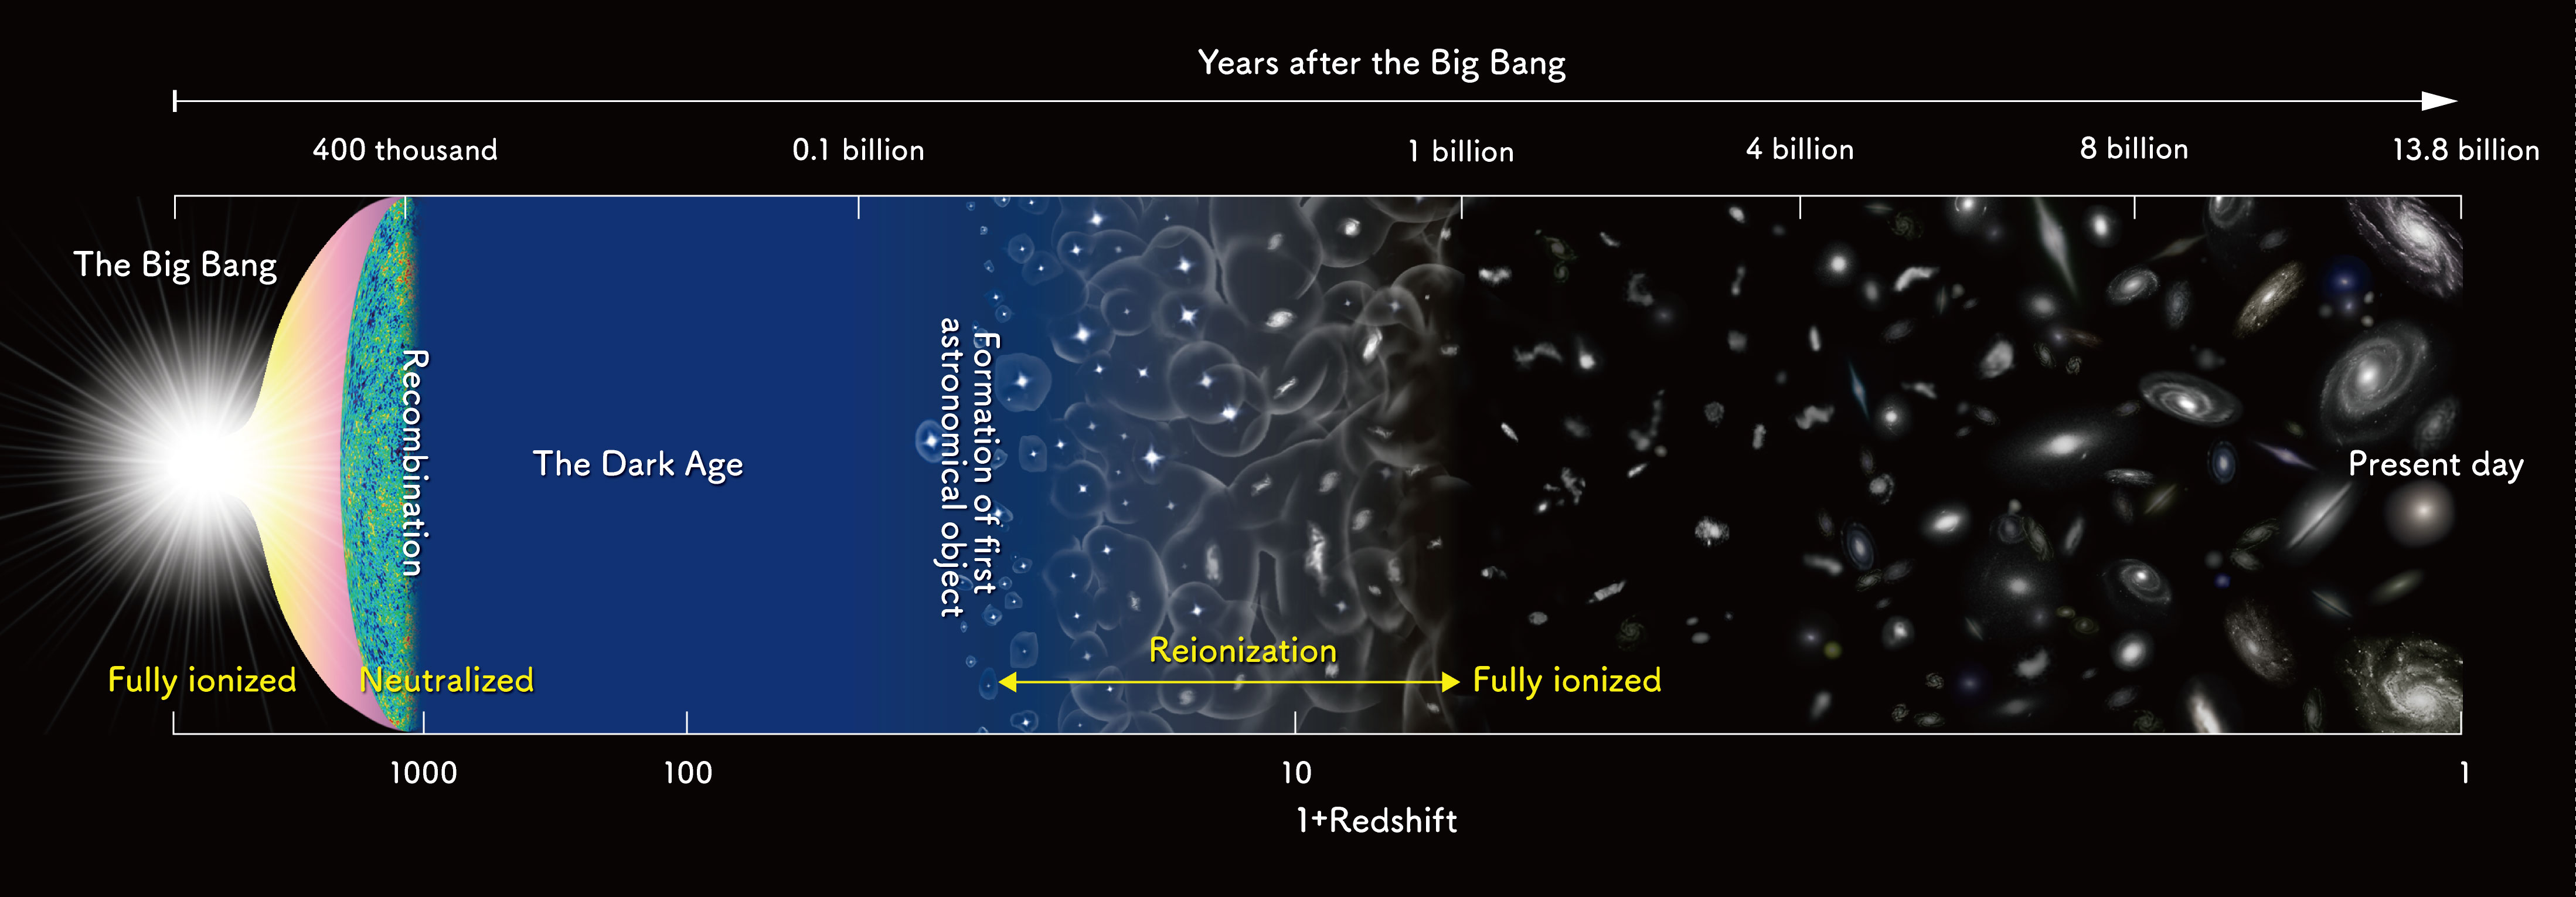
\includegraphics[width=.9\textwidth]{cosmic-applepie-cooking-time.jpg}
\caption{Illustration showing the approxiate time needed until applepie ingredients appear.}
\end{figure}

\begin{wrapfigure}{r}{0.15\textwidth}
    \centering
    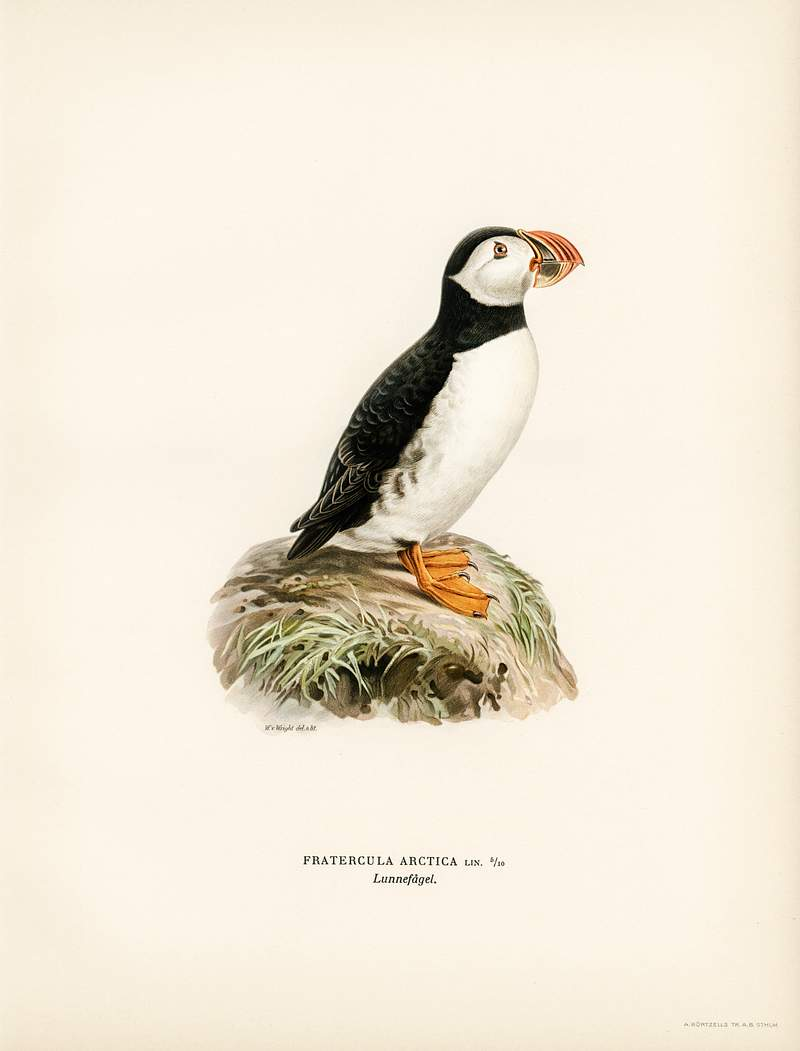
\includegraphics[width=.15\textwidth]{puffin.jpg}
\end{wrapfigure}

Assuming, you wait for grocery stores to appear, collect these from the nearest one.

With your standard kitchen utilities, mix the collected items and bake until ready.

Enjoy with your fellow human beings.

Bon appetit

\end{document}
